\documentclass[aspectratio=169]{beamer}

% =========================
% TEMA
% =========================
\usetheme{Madrid}
\usecolortheme{default}

% =========================
% PAQUETES
% =========================
\usepackage[spanish,es-nodecimaldot]{babel}
\usepackage[utf8]{inputenc}
\usepackage[T1]{fontenc}
\usepackage{amsmath,amssymb}
\usepackage{graphicx}
\usepackage{booktabs}
\usepackage{circuitikz}

% =========================
% INFORMACIÓN
% =========================
\title{Diseño e implementación de un control óptimo}
\subtitle{Producto Integrador de Aprendizaje}
\author{Gabriel González Alvarez}
\institute{
Universidad Autónoma de Nuevo León\\
Facultad de Ingeniería Mecánica y Eléctrica
}
\date{Mayo 2026}

% =========================
\begin{document}

% =====================================================
\begin{frame}
\titlepage
\end{frame}

% =====================================================
\begin{frame}{Contenido}
\tableofcontents
\end{frame}

% =====================================================
\section{Introducción}

\begin{frame}{Introducción}

\begin{itemize}
\item Se desarrolló el modelado matemático de un sistema RC.
\vspace{0.3cm}

\item El sistema fue representado en espacio de estados.
\vspace{0.3cm}

\item Se diseñó un controlador óptimo LQR mediante la ecuación algebraica de Riccati.
\vspace{0.3cm}

\item Se comparó experimentalmente con:
\begin{itemize}
    \item Asignación de polos
    \item Control integral por asignación de polos
    \item Control LQI
\end{itemize}

\vspace{0.3cm}

\item La implementación experimental se realizó utilizando un ESP32 y cuatro plantas RC equivalentes.

\end{itemize}

\end{frame}

% =====================================================
\section{Modelo del sistema}

\begin{frame}{Sistema RC}

\begin{center}
\begin{circuitikz}[american, scale=0.75]
\draw (0,0) node[ground]{} 
to[V, l=$u(t)$] (0,4)
to[R, l=$R_1$] (3,4)
node[circ]{} node[above]{$V_1$}
to[C, l_=$C_1$] (3,0)
node[ground]{}

(3,4) to[R, l=$R_2$] (6,4)
node[circ]{} node[above]{$V_2$}
to[C, l_=$C_2$] (6,0)
node[ground]{}

(6,4) to[R, l=$R_3$] (9,4)
-- (9,0) node[ground]{};
\end{circuitikz}
\end{center}

\vspace{0.3cm}

\begin{itemize}
\item Variables de estado:
\[
x_1 = V_1, \qquad x_2 = V_2
\]

\item Salida:
\[
y = x_2
\]
\end{itemize}

\end{frame}

% =====================================================
\begin{frame}{Modelo en espacio de estados}

\[
\dot{x}=Ax+Bu
\]

\vspace{0.4cm}

\[
A=
\begin{bmatrix}
-\frac{1}{R_1 C_1} - \frac{1}{R_2 C_1} &
\frac{1}{R_2 C_1} \\
\frac{1}{R_2 C_2} &
-\frac{1}{R_2 C_2} - \frac{1}{R_3 C_2}
\end{bmatrix}
\]

\vspace{0.3cm}

\[
B=
\begin{bmatrix}
\frac{1}{R_1 C_1} \\
0
\end{bmatrix}
\]

\vspace{0.3cm}

\[
y =
\begin{bmatrix}
0 & 1
\end{bmatrix}x
\]

\end{frame}

% =====================================================
\section{Índice de desempeño}

\begin{frame}{Índice de desempeño}

Se definió un criterio cuadrático de desempeño:

\[
J = \int_{0}^{\infty}
\left(
x^TQx + u^TRu
\right)dt
\]

\vspace{0.5cm}

Matrices utilizadas:

\[
Q=
\begin{bmatrix}
1 & 0 \\
0 & 5
\end{bmatrix}
\]

\vspace{0.3cm}

\[
R = 1
\]

\vspace{0.5cm}

\begin{itemize}
\item Mayor peso al seguimiento del estado \(x_2\)
\item Penalización del esfuerzo de control
\item Base del diseño LQR
\end{itemize}

\end{frame}

% =====================================================
\section{Controlador LQR}

\begin{frame}{Diseño del controlador LQR}

El controlador óptimo se obtuvo resolviendo la ecuación algebraica de Riccati:

\[
P = solve\_continuous\_are(A,B,Q,R)
\]

\vspace{0.4cm}

Ganancia LQR:

\[
K = R^{-1}B^TP
\]

\vspace{0.4cm}

Resultado obtenido:

\[
K=
\begin{bmatrix}
0.4142 & 0.4142
\end{bmatrix}
\]

\vspace{0.4cm}

Ley de control:

\[
u=-Kx+gr
\]

\end{frame}

% =====================================================
\section{Seguimiento de referencia}

\begin{frame}{Seguimiento mediante cambio de coordenadas}

Se empleó una ganancia de prealimentación para eliminar el error en estado estacionario.

\vspace{0.4cm}

Ley de control:

\[
u=-Kx+gr
\]

\vspace{0.5cm}

Ganancia de seguimiento:

\[
g=
\begin{bmatrix}
K & 1
\end{bmatrix}
\begin{bmatrix}
A & B \\
C & D
\end{bmatrix}^{-1}
\begin{bmatrix}
0\\
0\\
1
\end{bmatrix}
\]

\vspace{0.5cm}

\begin{itemize}
\item Convierte el problema de seguimiento en regulación
\item Garantiza seguimiento de referencia constante
\end{itemize}

\end{frame}

% =====================================================
\section{Implementación experimental}

\begin{frame}{Implementación experimental}

\begin{itemize}
\item Se construyeron cuatro plantas RC equivalentes.
\vspace{0.3cm}

\item Se utilizó un microcontrolador ESP32.
\vspace{0.3cm}

\item Se implementaron simultáneamente:
\begin{itemize}
    \item Asignación de polos
    \item Integral por asignación de polos
    \item LQR
    \item LQI
\end{itemize}

\vspace{0.3cm}

\item Se adquirieron datos mediante comunicación serial y Python.
\end{itemize}

\end{frame}

% =====================================================
\begin{frame}{Implementación física}

\begin{center}
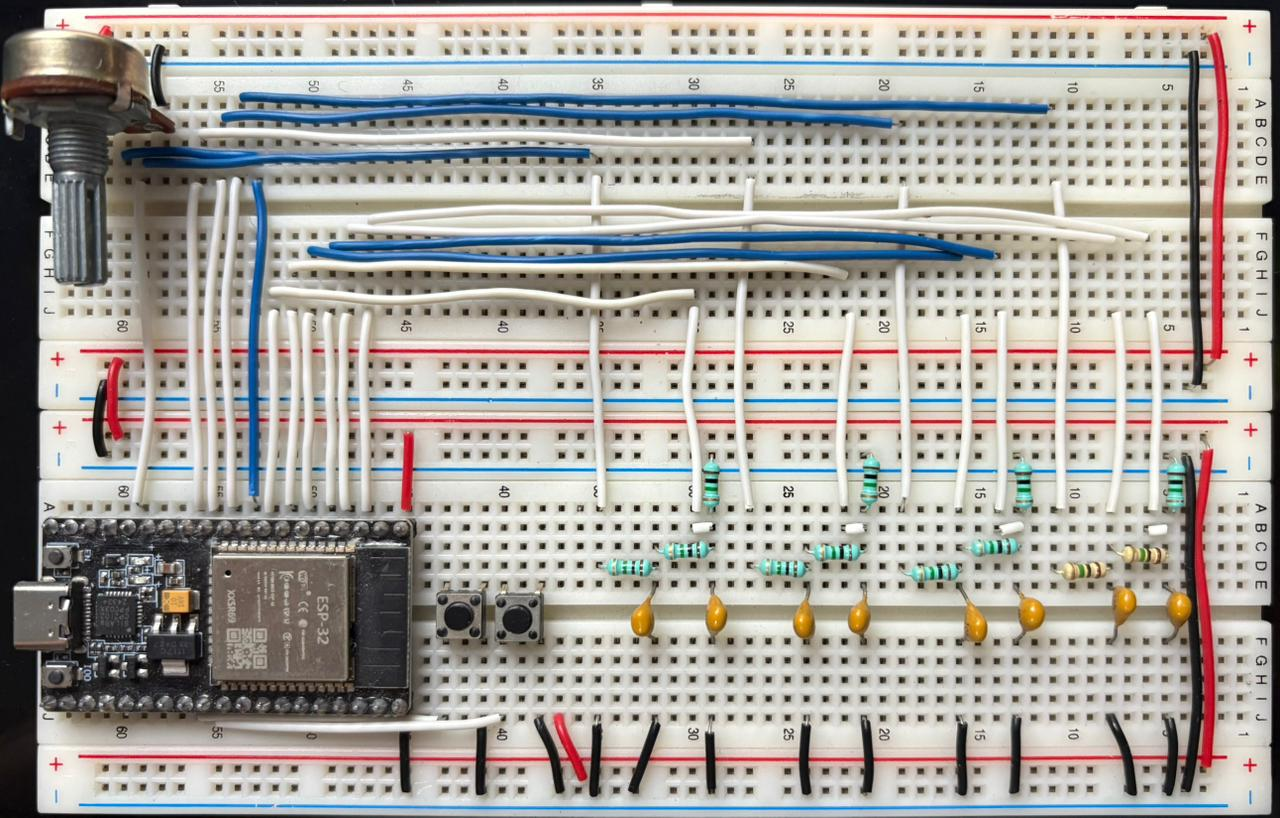
\includegraphics[width=0.7\textwidth]{Imagenes/proto.jpeg}
\end{center}

\end{frame}

% =====================================================
\section{Resultados experimentales}

\begin{frame}{Resultados experimentales}

\begin{center}

\includegraphics[width=0.7\textwidth]{Imagenes/reporte_monitor.png}
\end{center}

\end{frame}

% =====================================================
\begin{frame}{Comparación de desempeño}

\begin{table}[H]
\centering
\begin{tabular}{lc}
\toprule
Controlador & Índice \(J\) \\
\midrule
Asignación de polos & 181.51 \\
Integral AdP & 241.79 \\
LQR & 145.61 \\
LQI & 235.34 \\
\bottomrule
\end{tabular}
\end{table}

\vspace{0.5cm}

\begin{itemize}
\item El controlador LQR obtuvo el menor valor de \(J\)
\item Se verificó experimentalmente la optimalidad
\item LQI minimiza un funcional distinto sobre el sistema aumentado
\end{itemize}

\end{frame}

% =====================================================
\section{Conclusiones}

\begin{frame}{Conclusiones}

\begin{itemize}

\item Se obtuvo el modelo matemático del sistema RC en espacio de estados.
\vspace{0.3cm}

\item Se diseñó un controlador LQR mediante control óptimo.
\vspace{0.3cm}

\item Se implementaron estrategias adicionales:
\begin{itemize}
    \item Asignación de polos
    \item Integral por asignación de polos
    \item LQI
\end{itemize}

\vspace{0.3cm}

\item El controlador LQR presentó el mejor desempeño experimental.
\vspace{0.3cm}

\item Los resultados validan la minimización explícita del índice cuadrático como criterio de diseño.

\end{itemize}

\end{frame}

% =====================================================
\section{Referencias}

\begin{frame}{Referencias}

\footnotesize

\begin{thebibliography}{99}

\bibitem{Ogata}
K. Ogata,
\textit{Modern Control Engineering},
5th ed.,
Prentice Hall,
2010.

\vspace{0.3cm}

\bibitem{Kirk}
D. E. Kirk,
\textit{Optimal Control Theory: An Introduction},
Dover Publications,
2004.

\vspace{0.3cm}

\bibitem{Franklin}
G. F. Franklin, J. D. Powell, and A. Emami-Naeini,
\textit{Feedback Control of Dynamic Systems},
7th ed.,
Pearson,
2015.

\end{thebibliography}

\end{frame}

% =====================================================
\begin{frame}
\centering
\Huge
Gracias
\end{frame}

% =====================================================
\end{document}